\externaldocument{content/viewpoint}
\chapter{Registration of Superimposed Avatars \label{chap:registration}}
\begin{figure}[ht]
	\centering
	\subfloat[Superimposition registered at pelvis]{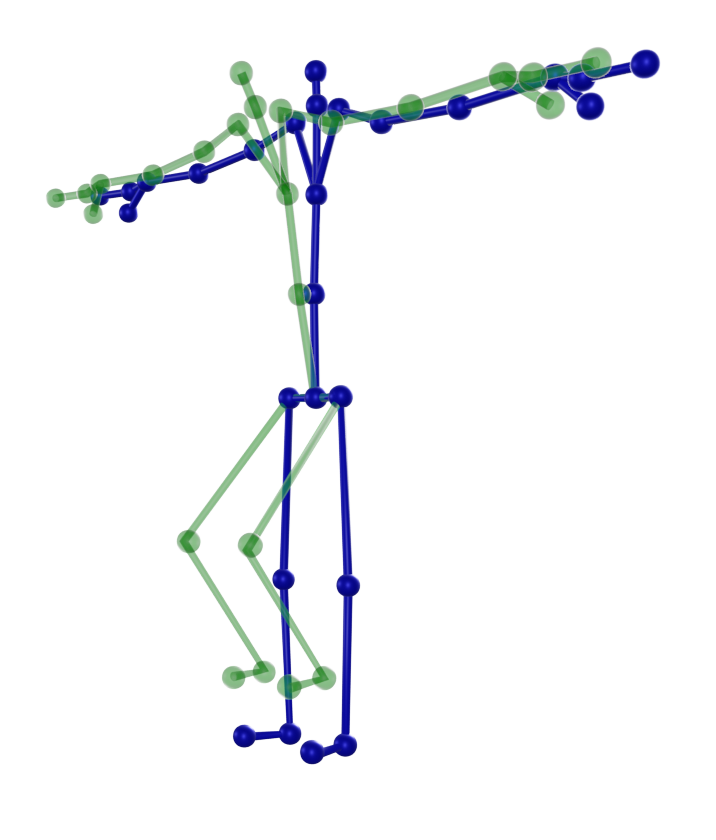
\includegraphics[height=0.35\linewidth]{pictures/pelvisReg.png}
		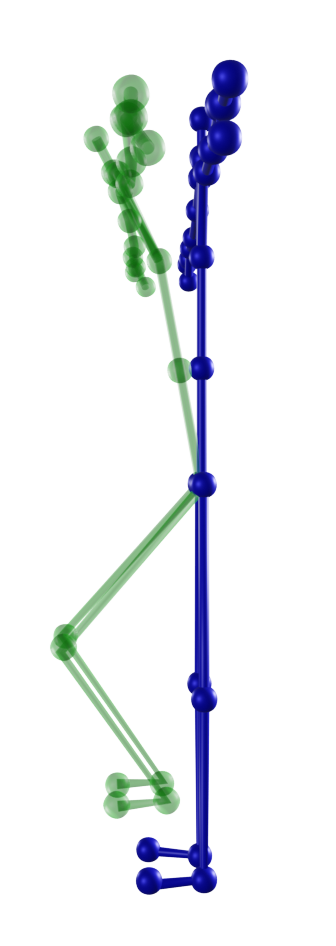
\includegraphics[height=0.35\linewidth]{pictures/pelvisRegSide.png}}
	\subfloat[Superimposition registered at feet]{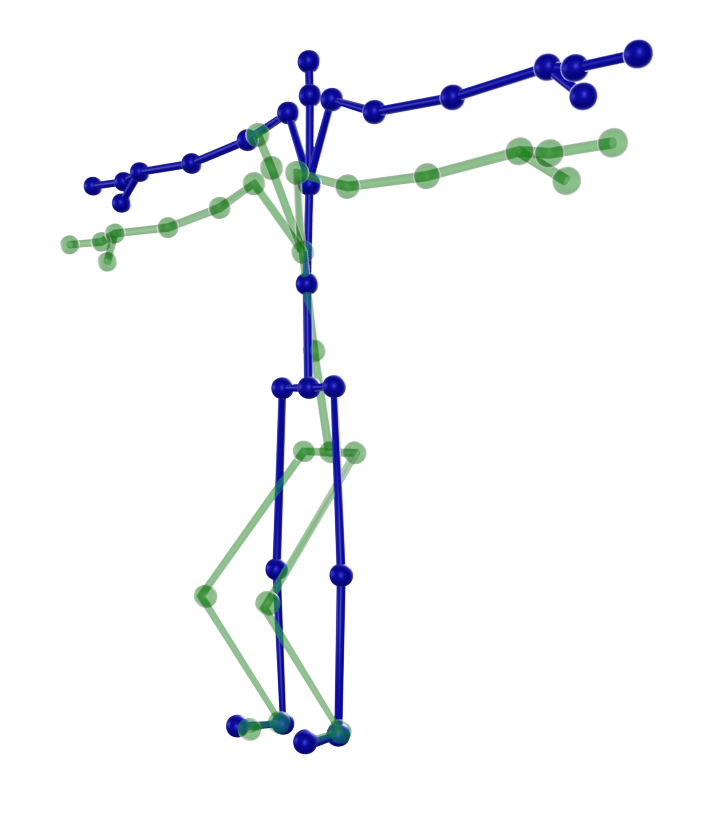
\includegraphics[height=0.35\linewidth]{pictures/footReg.png}
		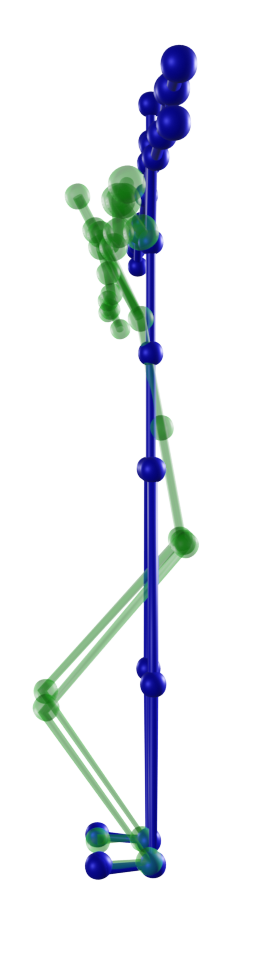
\includegraphics[height=0.35\linewidth]{pictures/footRegSide.png}}
	\caption[Illustrating the importance of registration.]{Illustrating the importance of registration: When registered at the pelvis (a), the squatting target avatar (in green) seems to be floating. Registering at the feet (b) seems to provide more intuitive feedback, connected to the environment.}
	\label{fig:registrationComparison}
\end{figure}

\section{Related Work \label{sec:relReg}}
In the current literature, we find a plethora of both rigid and non-rigid registration methods, as analyzed by Tam et al.~\cite{tam2012registration}. When registering an actual and target pose it is essential to use rigid registration, as we want to preserve potential deviations from the ideal form. These would be diminished by a non-rigid registration method, as it would deform the ideal avatar. Specifically for rigid registrations, there are several automatic methods, as Yaniv~\cite{yaniv2008rigid} and Bellekens et al.~\cite{bellekens2014survey} stated.

In some cases, a simple registration based on a single joint is completely sufficient. For example, for optimizing posture guidance in VR, Hoang et al.~\cite{hoang2016onebody} registered the target avatar based on the position and rotation of the pelvis. Instead, Anderson et al.~\cite{anderson2013youmove} used only the pelvis' position while maintaining the orientation of the recorded target movement. Subsequently, the approach was evaluated, and users performed two ballet and two abstract movements with the proposed system. In contrast, Naour et al.~\cite{naour2019superimpose} registered the avatars based on the position and rotation of the left foot. This way, the football-throwing motions of a learner were superimposed with those of an expert. Additionally, we find many approaches in the literature that register avatars but lack the explanation of methods.

\section{Methodology \label{sec:methReg}}
The registration of two exercises represents in most cases the foundation of visual feedback for motor skill training, in particular, superimposed avatars. When registering a superimposed actual and target avatar for a given exercise, we need to keep certain factors in mind to facilitate a better understanding of the scene for the user. For instance, the spatial relation of the avatars to the environment helps the user with orientation. Likewise, corrections for typical deviations have to be anticipated. In summary, a well-made registration can lead to a far more intuitive understanding of visual feedback.

The registration is directly linked to the other aspects of our feedback optimization. Not only does the registration directly influence the inputs of the \acrfull{pca} viewpoint calculation (i.e. $\Delta_n$ and  $\vec{v}_{Fn}$ in \autoref{eq:viewpoint} found in \autoref{sec:methViewCalc}), but it is a necessary prerequisite. Furthermore, our \acrshort{pca}-based viewpoint method as explained in \autoref{sec:methViewCalc}, is designed to work with smaller deviations. Therefore an appropriate registration method is important.

\subsection*{Optimal Avatar Registration \label{sec:optimalReg}}
An optimal avatar registration is highly dependent on the specific exercise performed and even on the individual interpreting the visual feedback. However, there are a few key aspects that are crucial in helping users to comprehend feedback using two superimposed avatars. In the following, we present guidelines, that can be used to register avatars for a certain scenario or to implement optimal avatar registration independently.

\begin{figure}[h]
	\centering
	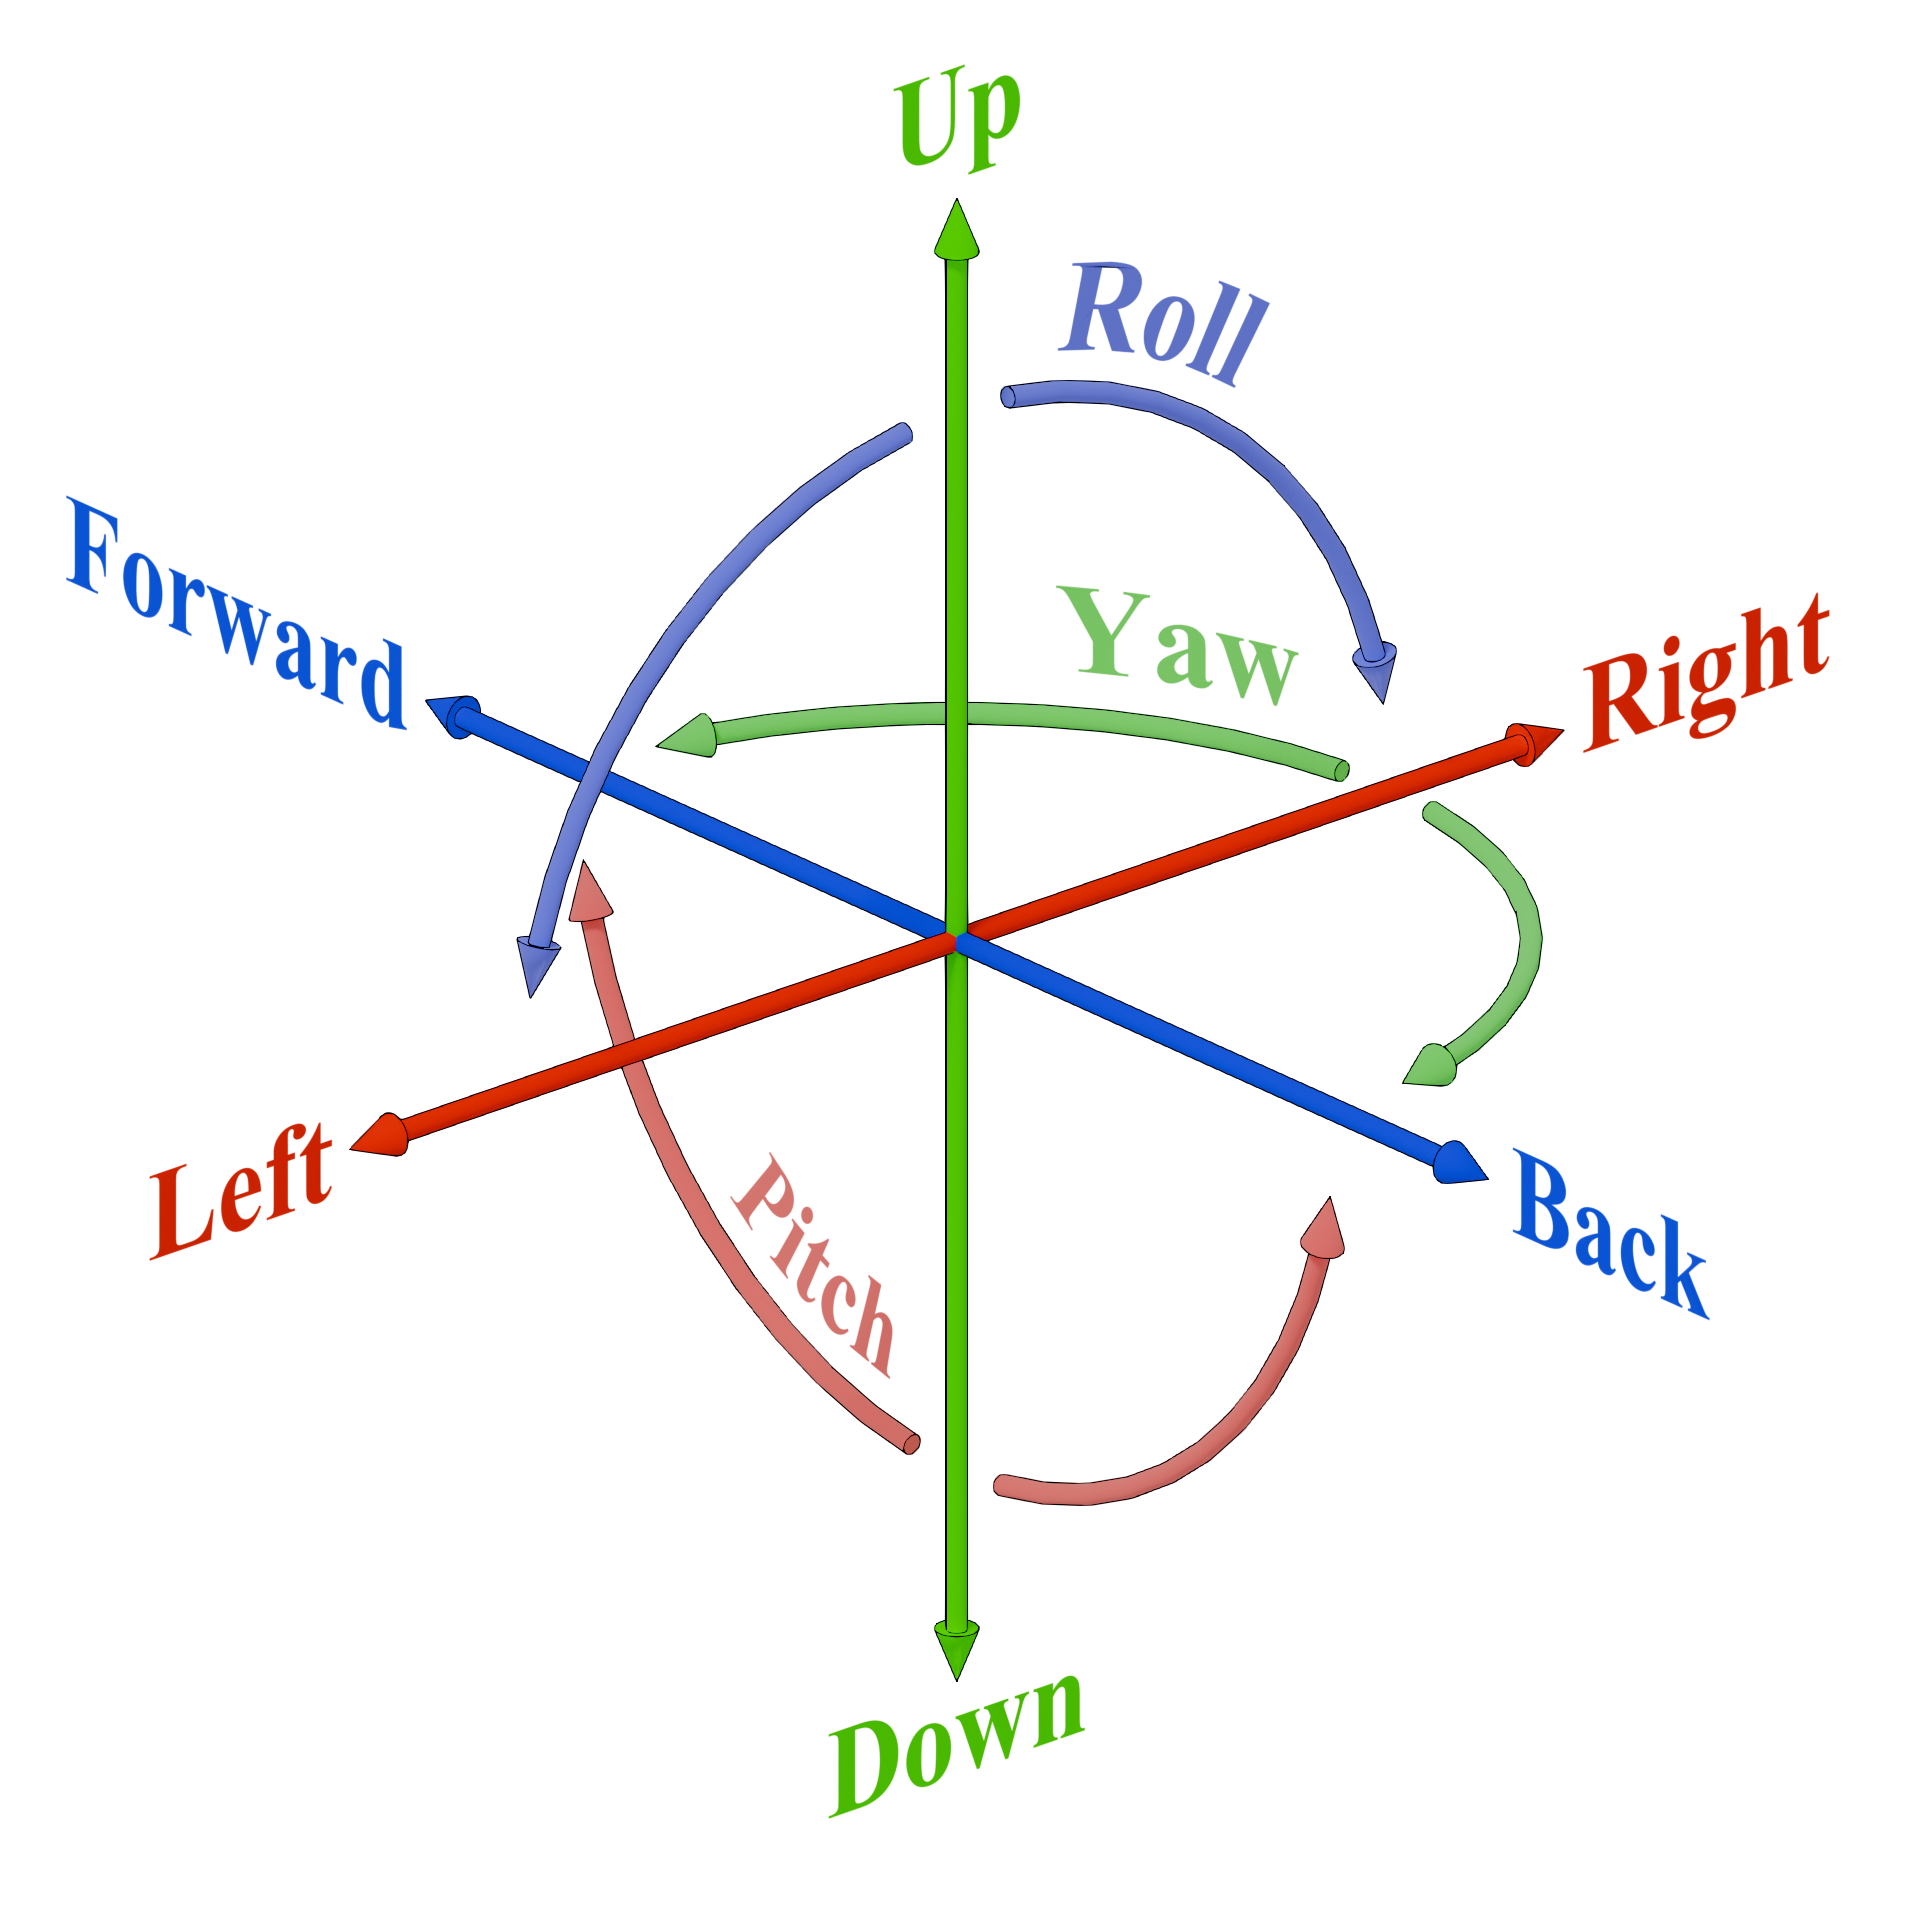
\includegraphics[width=0.5\linewidth]{pictures/Gizmos.png}
	\caption[Six degrees of freedom to define the placement of a rigid body.]{Six degrees of freedom to define the placement of a rigid body in space.}
	\label{fig:6dof}
\end{figure}

One single joint is oftentimes sufficient for registration. Especially for use cases with a limited selection of exercises, it can lead to satisfying results, as described in \autoref{sec:relReg}. However, to avoid irritating users it is important to connect the avatars with their spatial surroundings. For this purpose, we consider the six degrees of freedom (6DoF) for placing a rigid body in 3D space, as depicted in \autoref{fig:6dof}. We limited the 6DoF to four different categories, adequate to optimize registration:
\begin{itemize}
	\setlength{\itemsep}{-0.3cm}
	\item Vertical alignment (up/down)
	\item Horizontal alignment (left/right \& forward/backward)
	\item Rotation about vertical axis (yaw)
	\item Rotation about horizontal axes (pitch \& roll)
\end{itemize}

To provide the best avatar registrations, we match these 4 different degrees of freedom with the following characteristics from the fixed avatar:

\textbf{Vertical alignment:} As mentioned above, it is crucial to connect the target avatar to the environment. Otherwise, the user might be irritated, as the avatars seem to defy the rules of physics. Depending on the exercise, there are different connections to the surroundings: When doing exercises while standing like squats or lateral raises, the feet rest safely on the ground, thus connecting us with the environment. When hanging (e.g. pull-ups) or supporting the weight with the arms (e.g. dips) the hands connect us to the outer world. The user expects the target avatar to be connected to the environment the same way. Consequently, the connection to the environment represents a good measure of aligning the avatars. That means when the user is standing on the ground, the avatar squatting seems to do the same (see \autoref{fig:registrationComparison}). We can further improve the registration if the lowest point is matched for horizontal alignment. This way, when the user lifts a foot, the avatar still stays on the ground. Especially concerning exercises on the ground, this step leads to a better understanding of what to do, even when standing in a neutral position.

\textbf{Horizontal alignment:} The torso represents a big and important part of the body and also contains the center of mass while standing. Therefore, a horizontal alignment of both the actual and target avatars proved to be most intuitive based on the torso. Slightly better results can be achieved when choosing the point closest to the limbs connecting to the environment (i.e. the pelvis for standing exercises, a point between the shoulders for hanging, etc.).

\textbf{Rotation around vertical axis:}
The rotation around the vertical axis plays an important part in registering two avatars. In most cases, this rotation represents the orientation within the environment, which is arbitrary except when working with stationary equipment. This means the rotation around the vertical axis can be freely adapted without compromising the correct execution of an exercise. As mentioned in \autoref{sec:relReg}, there are a few joints with which the registration can seem intuitive, the joints in the torso emerge as the best option. In particular, using the same joint that we chose for the horizontal alignment delivers good results when also used as a reference for vertical rotation.

\textbf{Rotation around horizontal axes:}
During exercise performance, the rotation around the horizontal axes (i.e. pitching and rolling) is highly dependent on the exercise. Altering these rotations can lead to false interpretations of the feedback. Therefore, we see these rotations as exercise-inherent measures, which should not be altered (or only with great care). Consequently, the pitching and rolling rotations might best be carried over from the exercise recording or reference movement. Otherwise, the avatars seem too adaptive, possibly leading to wrong movement execution.

\subsection*{Scaling}
When two avatars are superimposed, depending on the recorded individuals, the scale of the limbs is not necessarily the same. Scaling one avatar according to the total size of the other avatar only partially solves the problem. As the proportions (e.g. torso length compared to leg length) can differ between individuals, a uniform scaling can still result in inconsistencies. Therefore, if the recorded exercises compared potentially stem from different individuals, it is advisable to scale the target avatar bone-wise to match the actual live avatar. Here, it is important to ensure that the angles between the bones, i.e. at the joints,  stay consistent. Otherwise, the scaling will falsify the exercise. 

\subsection*{Registration Limitations}
Avatar registration is a complex subject. The most generally applicable guidelines can be found above. However, it seems as if there is no optimal approach for every individual, situation, and use case. Especially when considering the details concerning the rotation around the horizontal axes, it seems in some cases there is a trade-off between the exercise's validity and perfect registration.
Furthermore, scaling the target avatar eliminates most inconsistencies in a bone-wise fashion, yet the angles between the bones at the joints stay consistent. Consequently, given certain proportions and thus centers of mass of two individuals compared, the scaling could lead to the target exercise not being the most optimal. Although the methods mentioned above yield good results for most exercises, even when registering with a neutral standing position, hanging exercises are hard to perceive while standing. This results from missing reference points of the environment. Once the actual avatar is hanging, we can use the hands as reference points (in particular, horizontal alignment).

\begin{figure*}[h]
	\centering
	\captionsetup[subfigure]{labelformat=empty}
	\subfloat[\centering Push-up (P)]{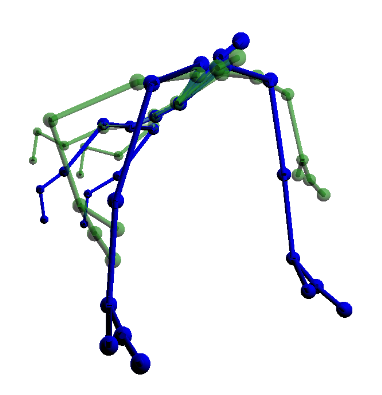
\includegraphics[height=.16\linewidth]{pictures/pushupPelvis.PNG}\hfill}  
	\subfloat[\centering Push-up (R)]{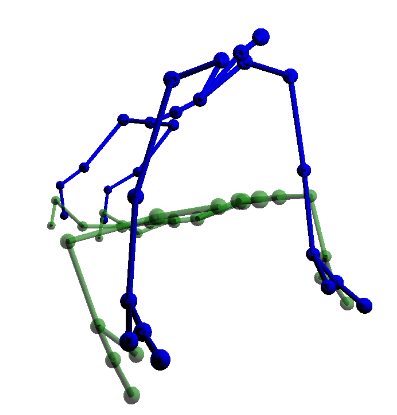
\includegraphics[height=.16\linewidth]{pictures/pushupRegistered.PNG}\hfill} 
	\subfloat[\centering Dip (P)]{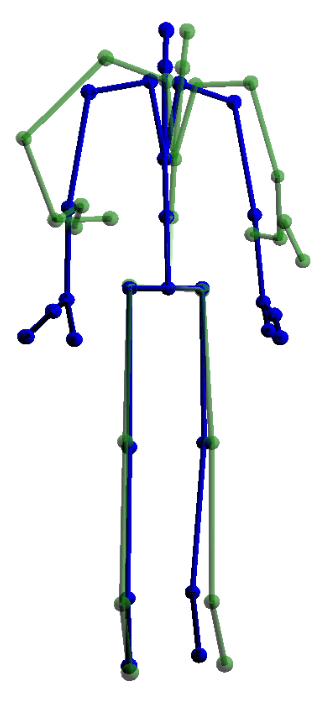
\includegraphics[height=.27\linewidth]{pictures/dipsPelvis.PNG}\hfill} 
	\subfloat[\centering Dip (R)]{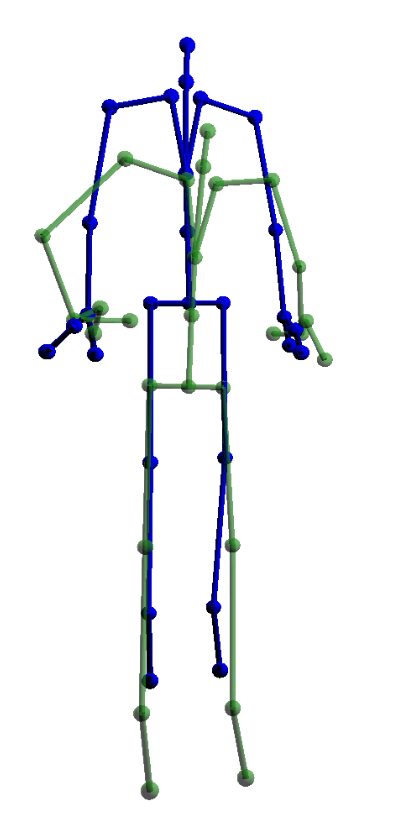
\includegraphics[height=.27\linewidth]{pictures/dipsRegistered.PNG}\hfill} 
	\subfloat[\centering Jump (F)]{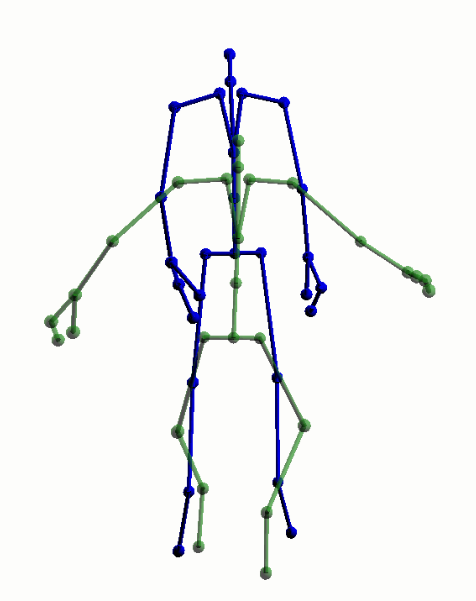
\includegraphics[height=.27\linewidth]{pictures/jumpFeet.PNG}\hfill}
	\subfloat[\centering Jump (R)]{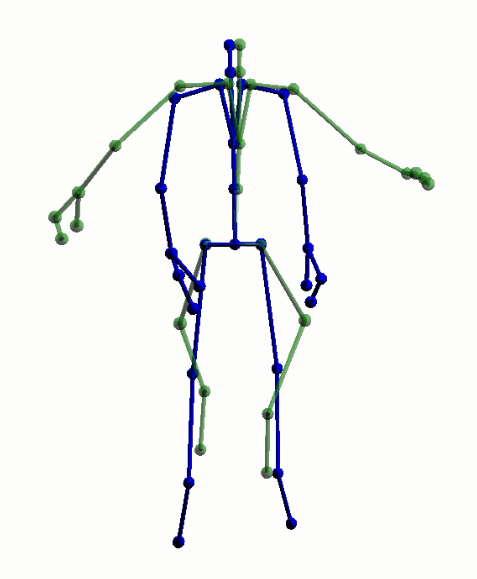
\includegraphics[height=.27\linewidth]{pictures/jumpPelvis.PNG}\hfill} 
	\caption[Registered start and execution position of exercise examples.]{Start and execution position of exercise examples registered according to our registration methods explained in \autoref{sec:optimalReg} (R), the feet (F) and only the pelvis (P). The exercises and registration parameters can be found in \autoref{tab:regExamples}.}
	\label{fig:regExamples}
\end{figure*}

\subsection*{Examples \label{sec:regExamples}}
To establish an understanding of the methods explained in \autoref{sec:optimalReg}, we chose a few exercises with corresponding joints to match the six degrees of freedom and will discuss them in this section. The exercises can be seen in \autoref{fig:regExamples} and the joints used for alignment can be taken from \autoref{tab:regExamples}. The examples were each chosen to be representative of a category of exercises. They are not meant to be complete, but rather a diverse collection, where finding examples close to many use cases is possible. Regarding registration, the example exercises could be sorted into 3 categories, as seen in \autoref{tab:regExamples}, based on how the individual connects with the environment:

\textbf{Connection to floor:}
Exercises that connect with the feet on the floor (like squats and warrior II), and those that involve lying down (like leg raises, plank, and push-ups) both profit from the same registration. Here, the pelvis was used to align the avatars on the horizontal plane. As a result, the torsos and therefore, the body's center were registered quite well. The avatars were vertically placed by aligning the lowest joint of each. Consequently, the avatars were intuitively placed on the floor, even if the movement of the actual avatar did not (yet) follow the target avatar (see \autoref{fig:regExamples} and \autoref{fig:registrationComparison}). Concerning rotation, the pitch and roll rotations, as depicted in \autoref{fig:6dof}, were fixated as in the recorded exercise. As already stated in \autoref{sec:optimalReg}, the pitch and roll rotations seem inherent to the exercise, as altering them can falsify the execution. However, the yaw rotation was based on the same joint used for horizontal alignment: The pelvis. This aligns the main orientations of the avatars.

\begin{table}[h]
	\caption[Example exercises with corresponding registration.]{Exercise examples with corresponding joints for each of the six degrees of freedom to match for an optimized registration as described in \autoref{sec:optimalReg}.\label{tab:regExamples}}
	\footnotesize
	\begin{tabular*}{\textwidth}{@{\extracolsep\fill}lcccccc}
		\toprule%
		& \multicolumn{3}{@{}c@{}}{Translation along} & \multicolumn{3}{@{}c@{}}{Rotation around} \\\cmidrule{2-4}\cmidrule{5-7}
		& \multicolumn{1}{@{}c@{}}{Vertical axis} & \multicolumn{2}{@{}c@{}}{Horizontal axes} & \multicolumn{1}{@{}c@{}}{Vertical axis} & \multicolumn{2}{@{}c@{}}{Horizontal axes} \\\cmidrule{2-2}\cmidrule{3-4}\cmidrule{5-5}\cmidrule{6-7}
		Exercise & Up/Down & Left/Right & Forward/Back & Yaw & Pitch & Roll\\
		\midrule
		Squat  & Lowest Joint & Pelvis & Pelvis & Pelvis & Fixed & Fixed\\
		Leg raise  & Lowest Joint & Pelvis & Pelvis & Pelvis & Fixed & Fixed\\
		Push-ups  & Lowest Joint & Pelvis & Pelvis & Pelvis & Fixed & Fixed\\
		Warrior II  & Lowest Joint & Pelvis & Pelvis & Pelvis & Fixed & Fixed\\
		Plank & Lowest Joint & Pelvis & Pelvis & Pelvis & Fixed & Fixed\\
		Dips  & Hands & Neck & Neck & Neck & Fixed & Fixed\\
		Pull-up  & Hands & Neck & Neck & Neck & Fixed & Fixed\\
		Jump  & Pelvis & Pelvis & Pelvis & Pelvis & Fixed & Fixed\\
		\bottomrule
	\end{tabular*}
\end{table}

\textbf{Connection to equipment:}
Alternatively, during an exercise, the individual could connect with the environment on a piece of equipment. For example, this is the case when doing dips or pull-ups where the individual is either supported or suspended by the arms, as seen in \autoref{fig:regExamples}. As a joint for both, horizontal alignment as well as yaw alignment, the base of the neck (i.e. center between shoulders) was chosen. Here, this provides a more intuitive registration point than the pelvis, as the arms connect to the environment. For the same reason, the hands were chosen as the base for a vertical alignment. Since the bars for dips or pull-ups represent the connection to the environment, registration at the hands appears stable and intuitive.

\textbf{No connection to the environment:}
Lastly, some exercises require no connection to the environment (like jumping or swimming). Still, it is possible to register avatars in these cases. To do so, the pelvis is chosen as the center of the body, as seen in \autoref{fig:regExamples}. The pitch and roll rotations are again fixated on the target avatar from how the exercise was recorded. The remaining alignments (i.e. up/down, left/right, forward/backward, yaw) are all done according to the pelvis.